\documentclass[12pt,a4paper,twoside]{article}

\setlength{\oddsidemargin}{-0.4mm}    % 25 mm left margin - 1 in
\setlength{\evensidemargin}{\oddsidemargin}
\setlength{\topmargin}{-5.4mm}        % 20 mm top margin - 1 in
\setlength{\textwidth}{160mm}         % 25 mm right margin
\setlength{\textheight}{247mm}        % 20 mm bottom margin
\setlength{\headheight}{5mm}
\setlength{\headsep}{5mm}
\setlength{\parindent}{0mm}
\setlength{\parskip}{\medskipamount}
\usepackage[pdftex]{graphicx}
\newcommand{\HRule}{\rule{\linewidth}{0.5mm}}
\usepackage{float}
\usepackage{bigstrut}
\usepackage{array}
\usepackage{graphicx}
\usepackage{epstopdf}
\newenvironment{myindentpar}[1]%
 {\vspace{-2mm}\begin{list}{}%
         {\setlength{\leftmargin}{#1}}%
         \item[]%
 \vspace{-2mm}}
 {\end{list}}
\raggedbottom


\begin{document}

% Title page
\begin{titlepage}
\begin{center}
% Upper part of the page
%
\includegraphics[scale=0.1]{camlogo.jpg}\\[1cm]    


\textsc{\LARGE University of Cambridge}\\[3.5cm]

\textsc{\Large Computer Science Tripos \\[2mm] Part 1B Group Project}\\[0.4cm]
\textsc{\Large Team Foxtrot - Race the Wild}\\[2cm]


%\HRule \\[0.4cm]
{ \huge \bfseries \vspace{3.5mm} Progress Report }\\[2cm]

%\hrule \\[1.9cm]

\begin{center}
\large
Sam Ainsworth\\
Ciaran Deasy\\
Matthew Ireland\\
Tom McCarthy\\
Andrew Sheriff\\
Christopher Wheelhouse\\
\end{center}

\vfill

% Bottom of the page
{\large Last Revised: \today}
\end{center}
\end{titlepage}

\newpage
\pagestyle{empty}
\cleardoublepage                             % so it actually prints out nicely doubleside!
\newpage

% Main document
\section{Overview}

Development of the Race the Wild app has so far been successful. 
The first prototype was delivered on-time, with a slightly different feature set to what was planned, and a demonstration video was made available to showcase the functionality. 
As of the time of writing, the second prototype has been completed, and will be tested before being demonstrated live at the client meeting on Friday Feb 15th. 
This prototype is almost feature-complete, as described in the requirements. 
Further refinements in the third iteration will yield a full product, leaving the final week for content creation and extensive testing and debugging.

\section{Progress}

\subsection{Features}

The second prototype broadly contains all of the features described in the requirements document. 
The menus, node map, scroll map, animal collection, position tracking and check-in systems are all accessible and functional. 
Some of these features are in need of refinement: in particular, the GPS tracking is complex and will require further attention before being considered acceptable to ship. 
However, everything has been implemented in some reasonable form.

Taking into account client feedback, some extra features are planned to be added.
\begin{itemize}
\item A simple challenge-based system. 
The player will be issued a challenge to move a certain distance in a certain time. 
If accepted and completed, the player will unlock animals which cannot be accessed by the standard ``check-in'' system.
\item An introduction and how-to-play system. 
The player will need to be instructed in how to use the app, and shown that their behaviour can earn them prizes. 
A short introduction will be provided when the app is first launched, and made accessible via the menu.
\end{itemize}

\subsection{Testing}

It was determined early in the project that the nature of the code was such that typical unit-testing would not be significantly helpful, due to it consisting of a lot of graphical code, as well as standard Android library systems, that needs to be manually tested by running the app in order to have confidence in its functional reliability. 
Thus, rather than taking the approach suggested in the initial Group Project briefing whereby modules would be unit-tested independently, the project was made to be runnable almost immediately. 
By adding code to a running program, the team could quickly and effectively get feedback as to whether any new code functioned correctly.

However, the team recognises the imperative need for structured and extensive testing of the product. 
To this end, an exhaustive manual test suite is to be written. 
Again, the team determined that the reliability of the product couldn't be measured confidently by automated methods. 
A combination of a rigorous formal test suite and ``typical'' use of the app from the perspective of end users will provide the soundest final product.

\section{Code Documentation}

The following sections, written individually by each group member, give documentation of the code written to date.

\subsection{Ciaran Deasy}

\subsubsection{Engine}

The Engine is the centre of the app. 
It stores references to the data structures like the Animal dictionary and Node list, and provides the interface by which components communicate. 
Directing such communication through the Engine simplifies other modules by keeping them independent. The Engine is also responsible for initial app setup.
The Engine is a singleton, and one is created at start-up.

\verb|static void initialise()|\\
Called at start-up. This will:
\begin{itemize}
\item Create the singleton Engine object.
\item Load the node data into a \verb|List| of \verb|Node|s.
\item Load the animal data into a \verb|Map| of \verb|(Integer, Animal)| pairs.
\item Load saved data, or create new data, as a \verb|PlayerStats| object.
\item Update all \verb|Animal|s and \verb|Node|s to be consistent with the data in the loaded/created \verb|PlayerStats| object.
\end{itemize}
Subsequent calls to this method will be ignored.

\verb|static void get()|\\
Returns the singleton \verb|Engine| object.

\verb|PlayerStats getStats()|\\
Returns the \verb|PlayerStats| object holding the player's current saved data.

\verb|List<Node> getNodeList()|\\
Returns the \verb|List| of all the \verb|Node| objects, containing data on each node in the game.

\verb|SatNavUpdate fetchSatNavData()|\\
Queries the GPS tracking service to get the latest movement information, which includes distance travelled and the movement point value. This is combined with the accumulated results of all previous queries since the player's last check-in, and the totals returned within a \verb|SatNavUpdate| object.

\verb|List<Animal> getAllAnimals()|\\
Returns a list of all the \verb|Animal| object, containing data on each animal in the game. The \verb|List| is sorted by animal ID.

\verb|Animal getAnimal(int ID)|\\
Returns the \verb|Animal| object containing data on the animal with the given \verb|ID|.

\verb|void changeColour(int animalID, Colour colour, Context c)|\\
Sets the \verb|Animal| with the given ID to have the given \verb|Colour| (\verb|Black| for found, \verb|Grey| for unfound, or \verb|White| for undiscovered). The animal will appear in the world, if not already present. Also updates the player's save data and saves it, which requires a \verb|Context| to access the filesystem.

\verb|void checkIn(Animal animal, Context c)|\\
Updates the given \verb|Animal| to be coloured \verb|Grey| (to indicate that it has been released), credits the player with movement points and distance accumulated since the last check-in, and saves player data, which requires a \verb|Context| to access the filesystem.

\verb|Node lookupNode(String name) throws NodeNotFoundException|\\
Returns the \verb|Node| object with the given name, which contains all data related to that node. Throws an exception if the name doesn't match any \verb|Node| in the game.

\subsubsection{Animal}

An object of the \verb|Animal| class encapsulates information about a particular animal in the game. A dictionary of these objects is created at program start and stored in the \verb|Engine|. 

\verb|int getID()|\\
Returns a unique ID for identifying the animal.

\verb|String getGraphicPath()|\\
Returns a filename for the animal's photo image in the filesystem, as displayed on the animal information screen.

\verb|String getSpritePath()|\\
Returns a filename for the animal's sprite image in the filesystem, as displayed in the game world.

\verb|String getName()|\\
Returns the name of the animal.

\verb|String getFacts()|\\
Returns the text description of the animal, as displayed on the animal information screen.

\verb|Node[] getNodes()|\\
Returns an array of the \verb|Node| objects representing the nodes in which the animal appears in the game world.

\verb|Colour getColour()|\\
Returns the colour of the animal.
\begin{itemize}
\item \verb|White| is the default, and corresponds to animals which haven't been discovered.
\item \verb|Grey| corresponds to animals that have been released into the wild, but not yet found by the player.
\item \verb|Black| corresponds to animals that the player has found.
\end{itemize}

\verb|String getHint()|\\
Returns the hint for this animal. This is displayed on the animal information screen when the animal has been released into the wild, but not yet found by the player, to provide a hint on the habitats in which the animal can be found.

\verb|int getDistancePerDay()|\\
Returns the distance in metres that the animal travels per day. Used to compare with the player's own movement on the check-in screen.

\verb|int compareTo(Animal other)|\\
A standard comparing method which compares animals by ID.

\verb|void setColour(Colour colour)|\\
Sets the animal to have a given colour (see \verb|getColour()|). Does NOT update other areas of the app, this must be handled by the caller.

\verb|Animal(int id, String name, String description, String hint, String graphic, |\\
\verb|    String sprite, int distancePerDay, List<String> nodeNames)|\\
Creates an animal with all the fields as provided above. The \verb|Colour| defaults to \verb|White|.

\subsubsection{Node}

An object of the \verb|Node| class encapsulates information about a particular habitat in the game, the regions on the world map that the player can visit. A list of these objects is created at program start and stored in the \verb|Engine|. 

\verb|String getName()|\\
Returns the name of this node. The name is used in code as a unique identifier for the node.

\verb|String getBackground()|\\
Returns the filename of the background image in the filesystem, which is shown when the node is visited.

\verb|String getPreview()|\\
Returns the filename of the preview image in the filesystem, which is shown on the node selection screen.

\verb|String getSprite()|\\
Returns the filename of the sprite in the filesystem, which is used to represent the node on the world map.

\verb|float getRelX()|\\
Returns a value between 0 and 1 to indicate the position of the node on the world map along the x-axis.

\verb|float getRelY()|\\
Returns a value between 0 and 1 to indicate the position of the node on the world map along the y-axis.

\verb|boolean hasName(String name)|\\
Returns true if the name of the node is the given name, and false otherwise. Isn't functionally different from testing manually, but gives rise to more readable code.

\verb|List<Animal> getAnimalList()|\\
Returns a list of all the animals that have been registered to appear in this node. This includes animals whose \verb|Colour| is grey or black, and which have this node in their list of habitats.

\verb|void addAnimal(Animal animal)|\\
Registers the given animal with this node. Registering an animal causes the animal to appear in this node when the player visits it. Only animals whose \verb|Colour| is grey or black, and which have this node in their list of habitats, should be registered with the node.

\subsubsection{XmlParser}

This abstract class provides static methods for creating the animal dictionary and node list at app start. The \verb|Engine| uses these methods as part of its initialisation process. All of the animal and node data is kept in XML files, and these methods provide the ability to parse these files to construct \verb|Animal| and \verb|Node| objects encapsulating the data.

\verb|static Map<Integer, Animal> createDictionary(XmlPullParser parser)|\\
\verb|    throws XmlReadException|\\
Returns a \verb|Map| of \verb|Animal| objects, keyed by the animals' ID fields. Android provides library support for opening XML files, and returns an \verb|XmlPullParser|. This parser can be provided to this method to be interpreted and turned into the required \verb|Animal| objects. If an error occurs during the parsing, an \verb|XmlReadException| will be thrown, with a \verb|message| describing the error encountered.

\verb|static List<Node> createNodes(XmlPullParser parser)|\\
\verb|    throws XmlReadException|\\
Returns a \verb|List| of \verb|Animal| objects. Android provides library support for opening XML files, and returns an \verb|XmlPullParser|. This parser can be provided to this method to be interpreted and turned into the required \verb|Node| objects. If an error occurs during the parsing, an \verb|XmlReadException| will be thrown, with a \verb|message| describing the error encountered.

\subsection{Sam Ainsworth \& Christopher Wheelhouse}


\subsubsection{BitmapDisplayAnimal implements Comparable}

This is the object used for drawing animals on the scrolling map. It simply stores data of each individual animal including its sprite, and has methods for drawing and collision detection.

\begin{verbatim}
BitmapDisplayAnimal(float xcoord, float ycoord, int animalCode,
 Bitmap bitmap, Colour colour)
\end{verbatim}

Creates a BitmapDisplayAnimal with all the fields as provided.

\begin{verbatim}
public void onDraw(Canvas c, float viewCenterx, float viewCentery, 
float screenWidth, float screenHeight)
\end{verbatim}

This is called in the drawing method of the scroll map. It calculates screen space coordinates of the animal and then displays it if it is on screen.

\verb£public boolean collisionCheck (float touchX, float touchY)£

Returns true if the position given to it collides with the image.

\verb£ public int compareTo(BitmapDisplayAnimal another)£

Used in sorting the animals when the first appear on screen.

\subsubsection{CollectionDisplayAnimal extends BitmapDisplayAnimal}

Like a BitmapDisplayAnimal, only with special methods to allow use of the features of the Collection screen.

\begin{verbatim}
BitmapDisplayAnimal(float xcoord, float ycoord, int animalCode,
 Bitmap bitmap, Colour colour, String bitmapName)
\end{verbatim}

Creates a CollectionDisplayAnimal with all the fields as provided.

\verb£ public int compareTo(BitmapDisplayAnimal another)£

Used in sorting the animals when the first appear on screen.

\verb£ public Boolean onScreen(float currentCenterY, £

 \verb£		 float screenWidth, float screenHeight)£

Returns true if the animal is currently on screen. Used to see if we can delete the animal's sprite from memory.

\verb£ public synchronized void onDraw(Canvas c, float currentCenterY,£

\verb£ 		float screenWidth, float screenHeight)£

Draws the image on screen if animal is in screen space, otherwise recycles the image. synchronized on Animal so that we don't recycle the image while actually drawing it.

\subsubsection{DisplayNode}

The graphics display class for nodes, on the NodeScene.

\begin{verbatim}
DisplayNode(float xcoord, float ycoord, Sting nodeName,
 Bitmap bitmap)
\end{verbatim}

Creates a DisplayNode with all the fields as provided.

\begin{verbatim}
public void onDraw(Canvas c, float viewCentery, 
float screenWidth, float screenHeight)
\end{verbatim}

This is called in the drawing method of the node map. It calculates screen space coordinates of the node and then displays it.

\verb£public boolean collisionCheck (float touchX, float touchY)£

Returns true if the position given to it collides with the image of the node.

\subsubsection{NodeScene extends Activity implements OnTouchListener}

This is the activity implementing the world map, used to navigate between habitats. It is implemented as an XML view, with an Android surface superimposed to do our custom drawing of the scrolling world map.

\begin{verbatim}
protected void onCreate(Bundle savedInstanceState)
\end{verbatim}

Initialises the Activity, retrieves the Engine, and gets data for nodes from it, which it then loads into DisplayNodes. Creates a SurfaceView for rendering on, then sets this as the viewpoint of the screen.

\begin{verbatim}
public void moveToScrollMap (View view)
\end{verbatim}

Called by the XML interface to move us to the scrolling habitat scenes. This method checks if we have selected a node, and if we have enough movement points to move to it, then sends us to the node screen.

\begin{verbatim}
public boolean onTouch(View arg0, MotionEvent arg1)
\end{verbatim}

This is called whenever the screen is touched. We check for collisions when a finger is put down on the screen, and scroll the screen when a finger is slid across it. If we touch a node, the selected node is changed, information is displayed about it, and a picture of that node is loaded and displayed.

\subsubsection{NodeViewer extends SurfaceView implements Runnable}

Inner class style used in the render-heavy scenes (NodeScene, ScrollAnimalCollection, ScrollMapScene) with similar implementations in each (called ScrollViewer in the others). This defines the specialised SurfaceView we use for rendering, along with particular iterations of methods suited for each style of NodeViewer in the system.

\verb£ public void pause()£

Called when the Android Pause state is reached. This stops rendering.

\verb£ public void resume()£

Called when the Android Resume state is reached. This resumes rendering.

\verb£ public void run()£

This is the graphics method, run in a separate thread to the updating of in game logic. It simply locks the drawing canvas, then calls the onDraw methods for all objects in the scene (particularly DisplayNodes in NodeScene), and unlocks the canvas again.


\subsubsection{ScrollAnimalCollection extends Activity implements OnTouchListener}

This is the activity implementing the animal collection, used to display animals we have discovered or found in game. It is implemented as a custom SurfaceView with the property that it only loads in sprites when they are on screen, since every animal could potentially be displayed in this scene.

\begin{verbatim}
protected void onCreate(Bundle savedInstanceState)
\end{verbatim}

Initialises the Activity, retrieves the Engine, and gets data for currently found animals, which it creates CollectionDisplayAnimals for but does not load animal images. At the end of the method, we call reloadAnimals, which loads all animals in the initial view point. 

\begin{verbatim}
private void reloadAnimals()
\end{verbatim}
This loads animals which are on screen but don't currently have an image in memory. It does this by synchronising on the animal (to avoid altering the Bitmap while it is being read) then loading in the Bitmap and setting a boolean flag to show this has been done. It is called whenever the screen is moved.


\begin{verbatim}
public boolean onTouch(View arg0, MotionEvent arg1)
\end{verbatim}

This is called whenever the screen is touched. We check for collisions when a finger is put down on the screen, and scroll the screen when a finger is slid across it. When the screen is scrolled, we reload animals on screen but without images, and when we touch an animal in the scene we move to the Animal Activity.

\subsubsection{ScrollViewer extends SurfaceView implements Runnable}

Inner class of ScrollAnimal Collection. Similar to the class in the NodeScene, but with altered implementation of run to call the specialised methods for the CollectionDisplayAnimals.


\subsubsection{ScrollMapScene extends Activity implements OnTouchListener}

This is the activity implementing the scrolling habitat maps, where we find the animals we have released using the check in system. It is implemented as a custom SurfaceView, which allows us to scroll around an image set in the current node parameters in PlayerStats, with the associated animals to that node, and set previously untouched animals as found in the event of touching them.

\begin{verbatim}
protected void onCreate(Bundle savedInstanceState)
\end{verbatim}

Initialises the Activity, retrieves the Engine, loads the background image, loads in animals (1 each of not yet found and 10 if already found) and places then in random positions on screen. The animals are then sorted according to y coordinate, to prevent them from standing on top of each other.

\begin{verbatim}
public void moveToCollection(View view)
\end{verbatim}
Allows us to move to the Animal collection on the press of a button onscreen. Called by the XML interface.

\begin{verbatim}
public boolean onTouch(View arg0, MotionEvent arg1)
\end{verbatim}

This is called whenever the screen is touched. We scroll the screen when a finger is slid across it. We check for collisions between the finger position and animals on-screen whenever a finger if first put down, and if it is an animal we haven't seen before we send the user to the screen with information about it, and set the animal as found. Unique to this class is the ability to scroll along both axes, meaning implementations differ compared to the other classes.

\subsubsection{ScrollViewer extends SurfaceView implements Runnable}

Inner class of ScrollMapScene Collection. Similar to the class in NodeScene, but calling local ScrollMap variables and using BitmapDisplayAnimals instead (thus justified over using a single outer class).





\subsection{Tom McCarthy}

\newpage
\subsection{Matthew Ireland - Design and implementation of location tracking subsystem}
\subsubsection{Theory \& Background}
The user's location needs to be periodically checked in order for them to acquire ``movement points" and for animals to be released into the virtual world. There are a number of interfaces available in Android for obtaining this data, but by far the most accurate method is to use the Global Positioning System (GPS). This accuracy does, however, come at the expense of an increase in power consumption and hence a decrease in battery life on the device upon which the app is running, so its use needs to be carefully controlled.

The user is awarded ``movement points'' based upon how far they move. However, a na\"{i}ve implementation could be exploited by users collecting large amounts of points by driving between cities, moving between countries by train or even flying to another continent. This kind of large, artificial movement is clearly not within the spirit of the application. A mechanism is therefore needed to avoid such pernicious malfeasance.

To distinguish different types of movement and award more points to distance travelled by bicycle and walking than by car and aeroplane, speed is taken into account and the number of movement points awarded is determined by the following equation:
\begin{equation}
\label{eq:mpoints}
M = \left({Ae^{-bv}+cv+d}\right)xe
\end{equation}
where $M$ is the number of movement points allocated for a given movement, $v$ is the average speed of the user over the period of the movement, $x$ is the distance travelled and $A$, $b$, $c$, $d$ and $e$ are coefficients whose values determine the precise allocation of movement points. How the use of this formula translates to real-world movement is shown in Figure 1, which shows at what rate movement points are allocated to with increasing speed for fixed distance, how far the user has to move to achieve a given number of movement points for increase speed and how long it would take a user to gain a given number of movement points with increasing speed as a result of application of the formula. The coefficients can be initially determined using numerical optimisation techniques and then further refined by taking into account empirical observations.

\begin{figure}
\centering
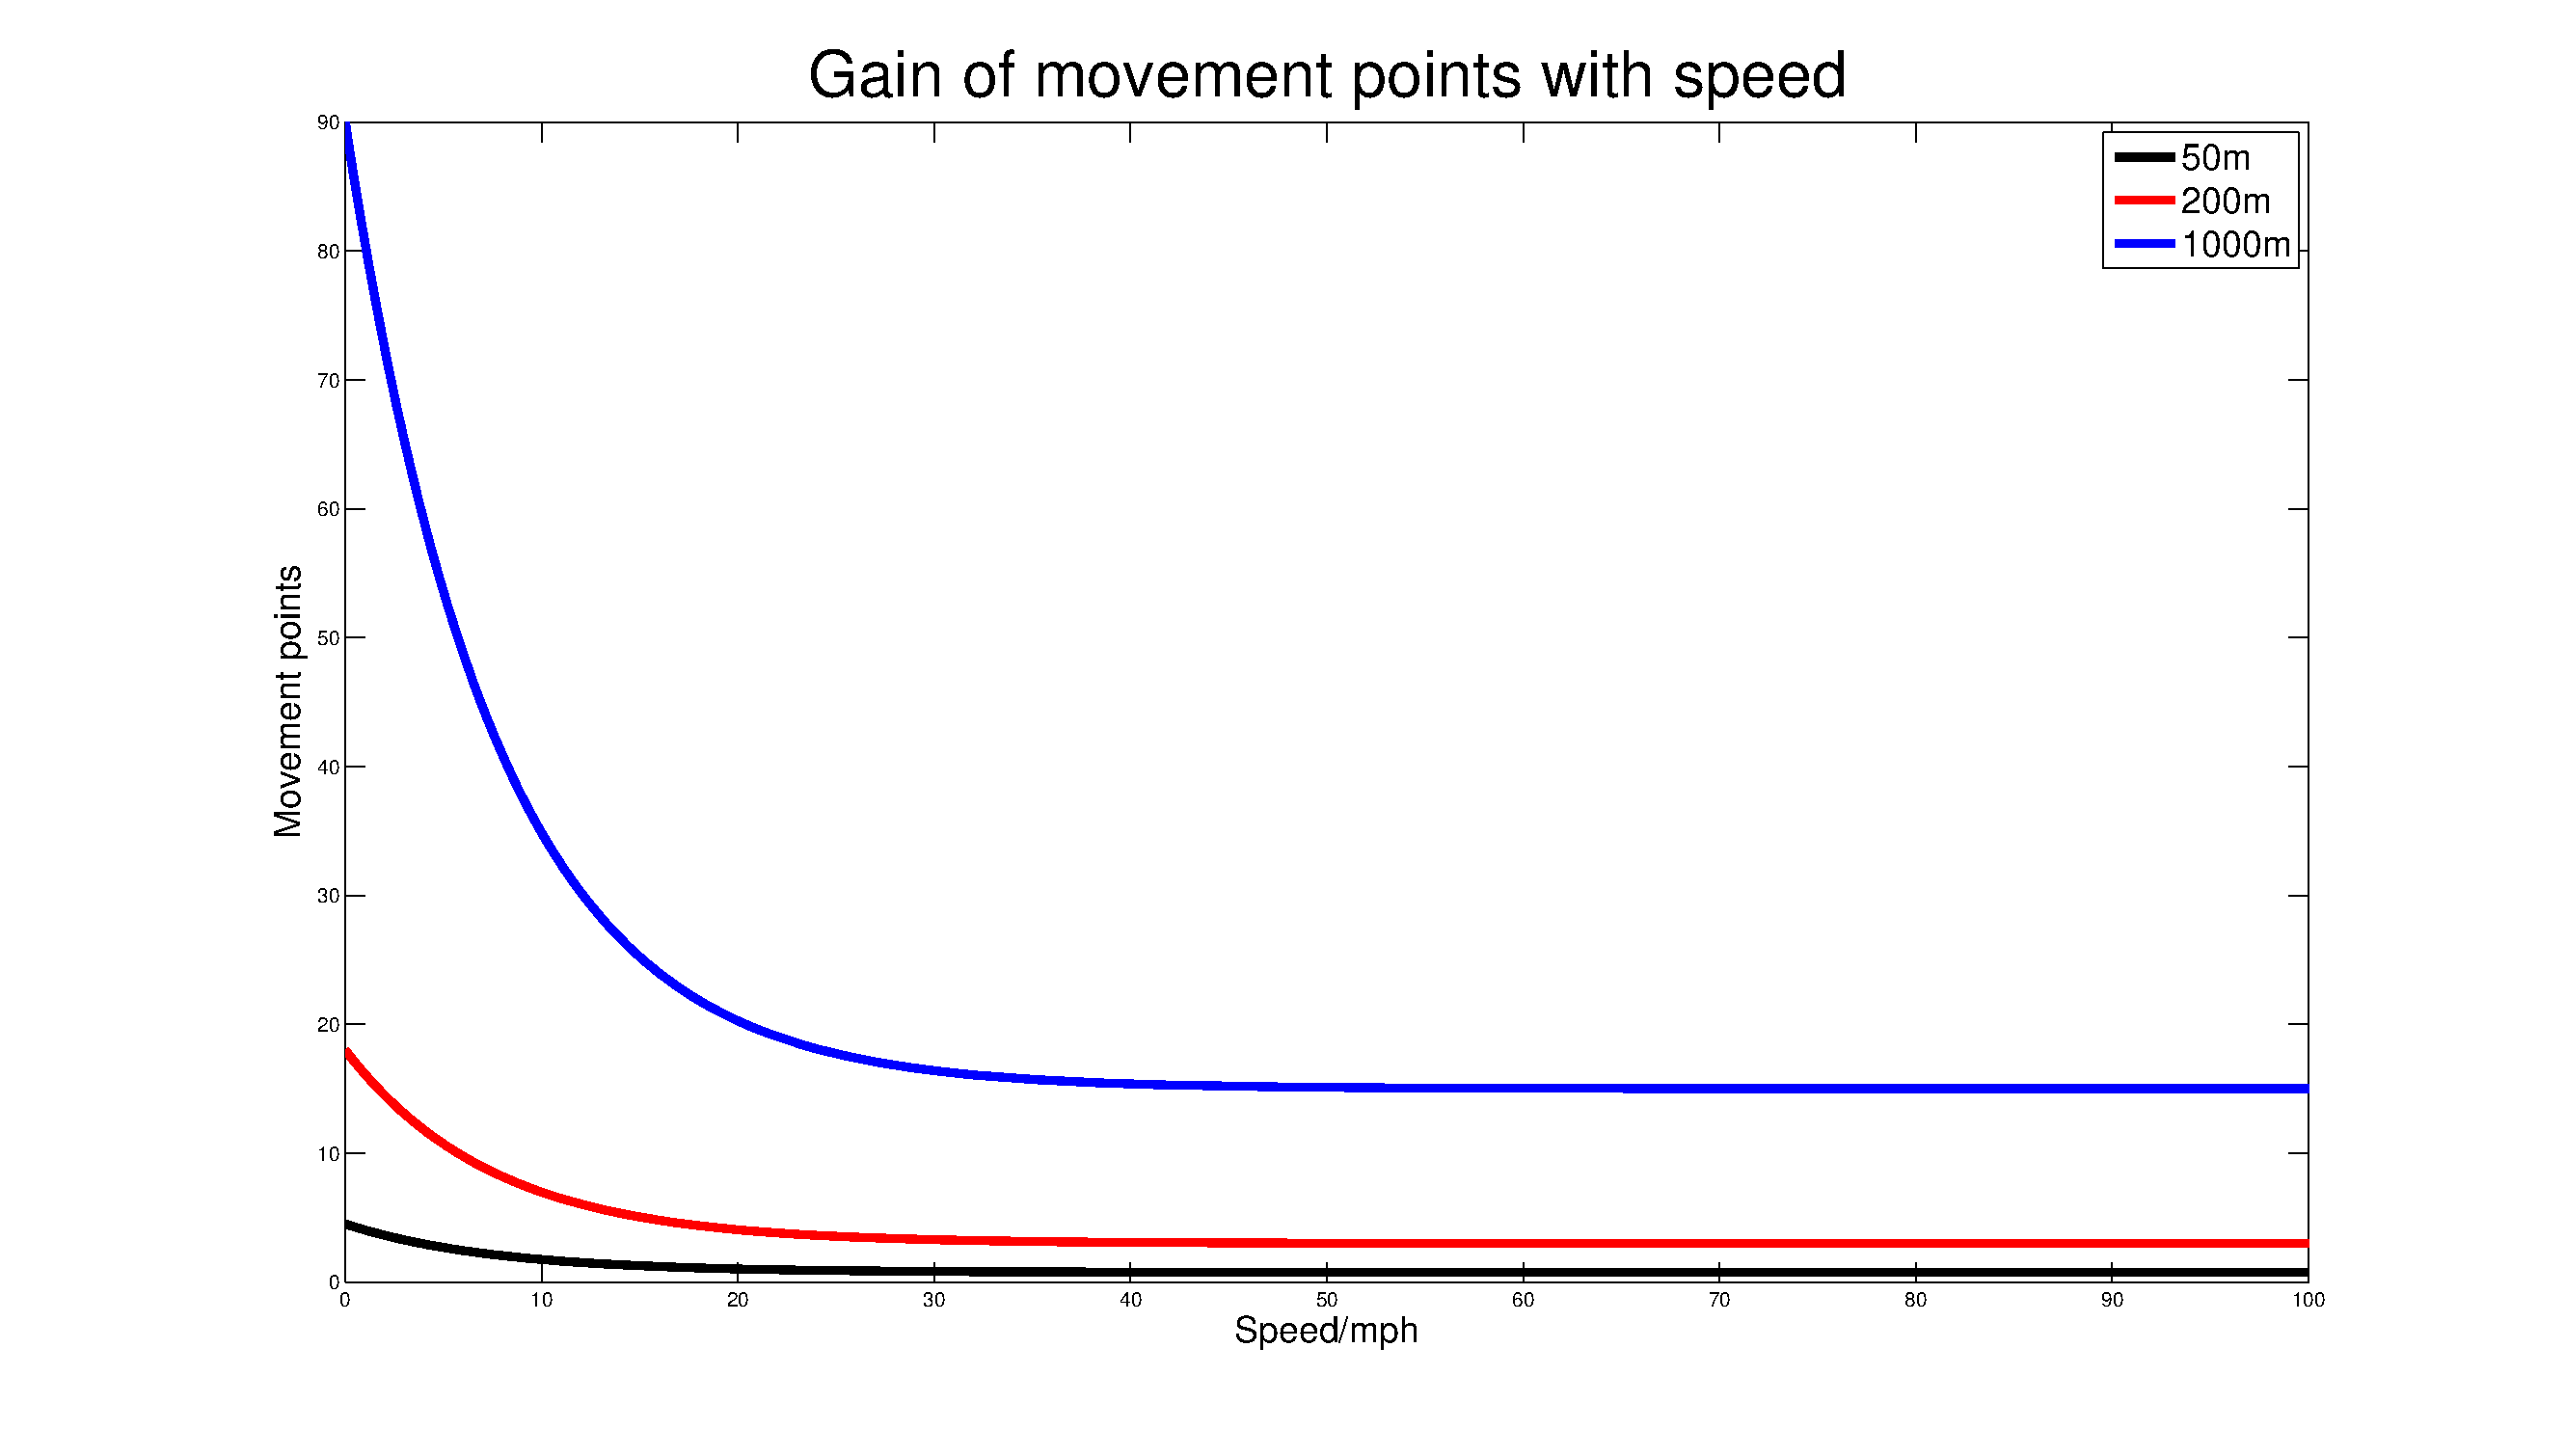
\includegraphics[scale=0.25]{m1.eps}

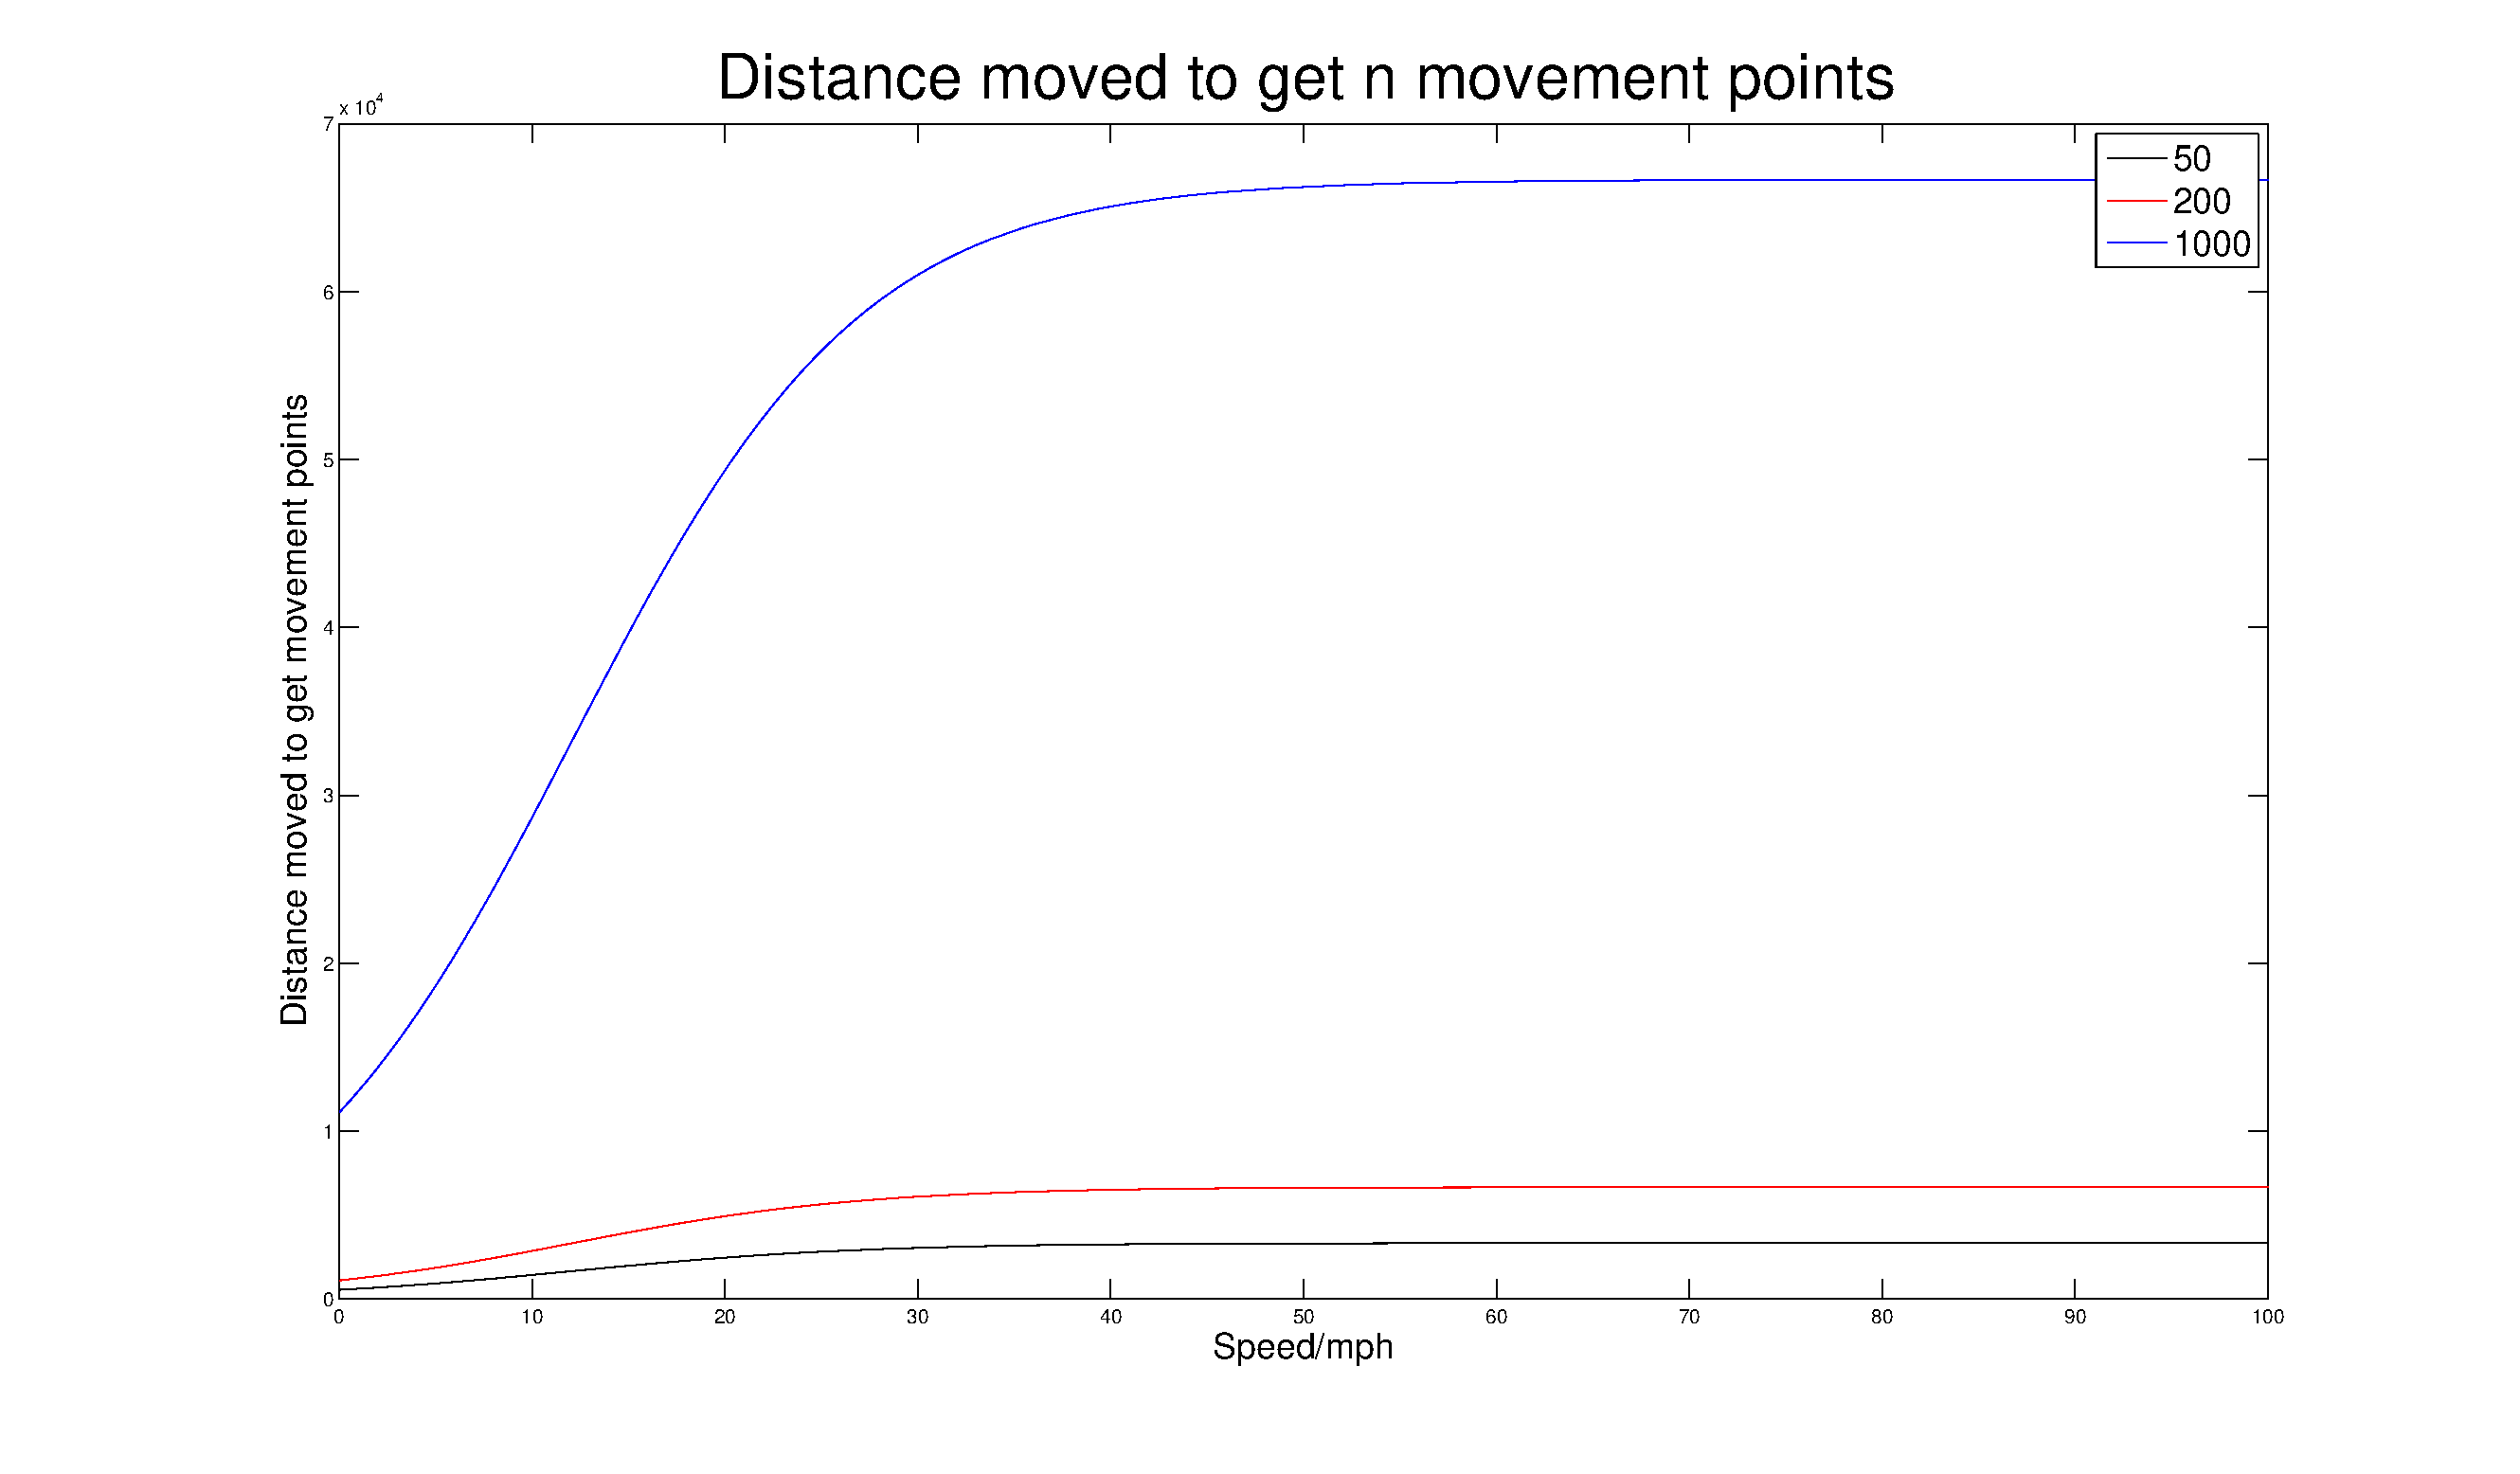
\includegraphics[scale=0.25]{m2.eps}

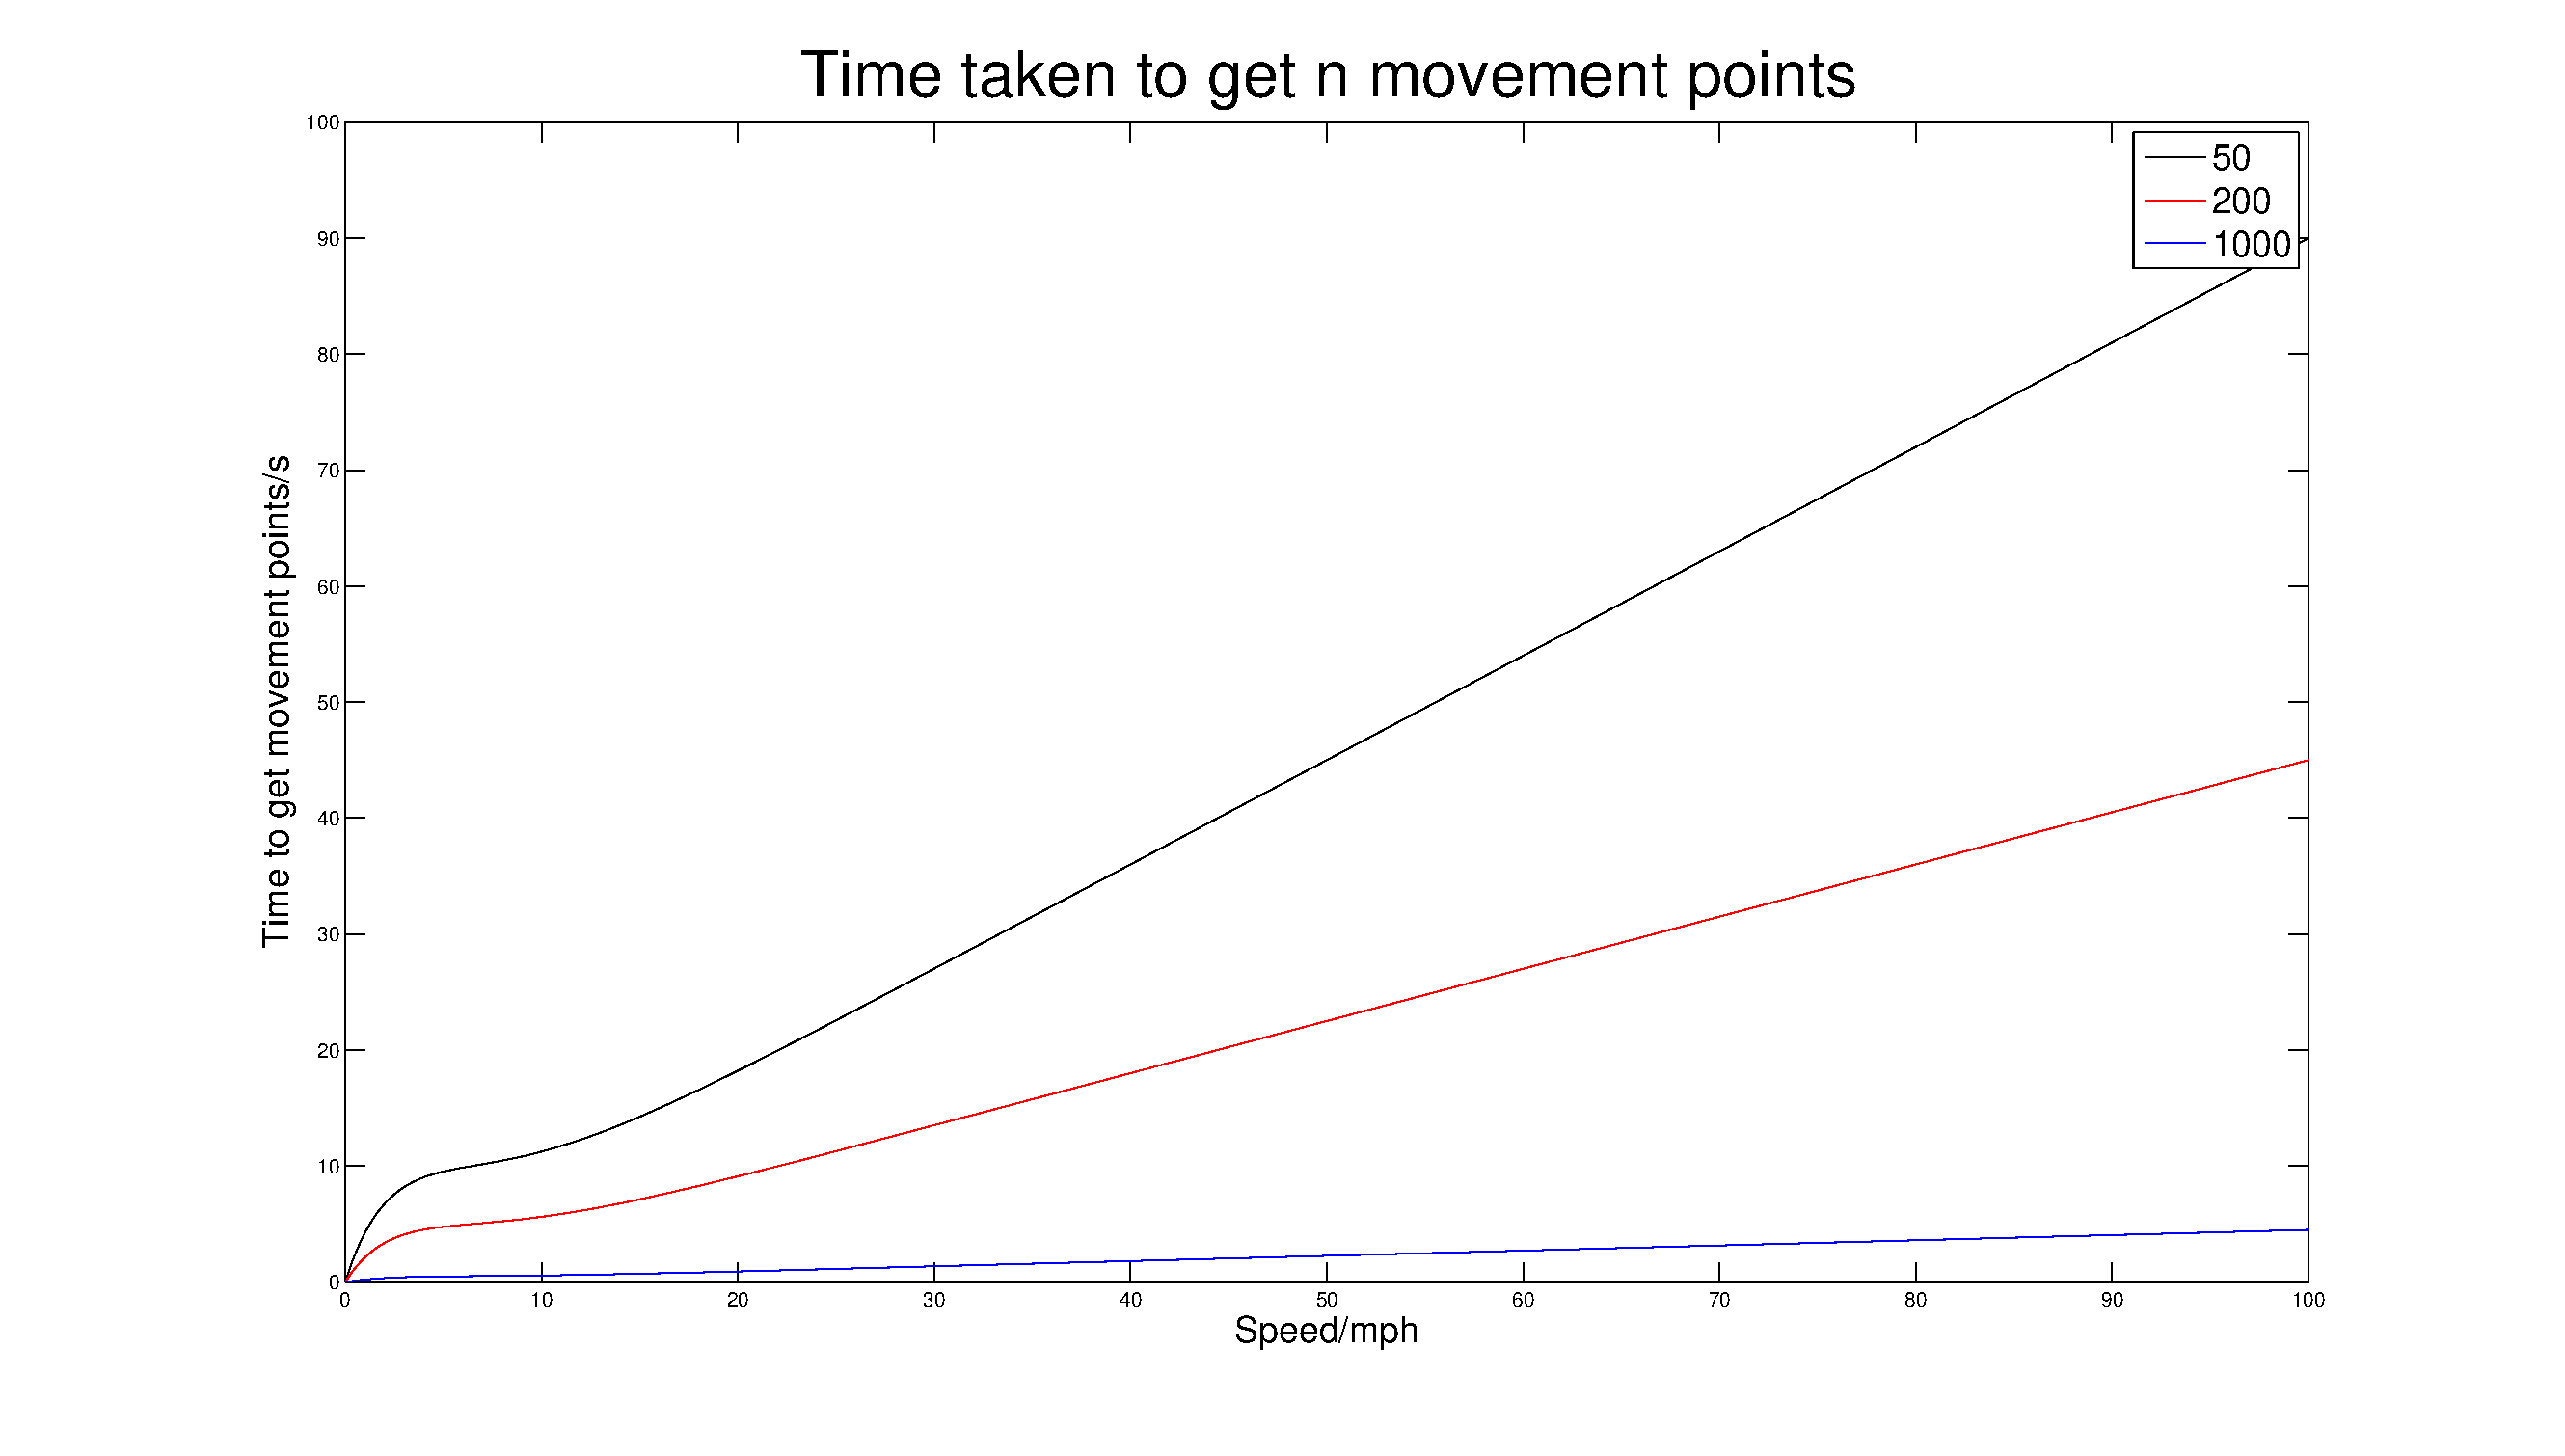
\includegraphics[scale=0.25]{m3.eps}

\caption{(left to right, top to bottom). The scales are fairly arbitrary at this stage of development. 1) Showing how the number of movement points awarded for travelling a given distance decreases with increasing speed. 2) Showing how far a user needs to move to gain a given number of movement points with increasing speed. 3) Showing how long it will take a user to gain a given number of movement points for increasing speed.}
\label{fig:movementeqn}
\end{figure}

\subsubsection{Overview of methods}
\textbf{public class GPSdebug extends Activity}\newline
\verb=GPSdebug= is the activity that provides an interface for initially starting the GPS and tweaking the coefficients of Equation \ref{eq:mpoints}.


\verb=public void startListeningToGPS(View view)=
\begin{myindentpar}{1cm}
This method reads the desired GPS poll time and uses the \verb=AlarmManager= Android system service to start the \verb=GPSservice= at regular intervals specified by this GPS poll time.
\end{myindentpar}

\verb=protected void onCreate(Bundle savedInstanceState)=
\begin{myindentpar}{1cm}
The old values of the movement point coefficients and GPS poll time are read from memory and displayed in the app to give the developer an opportunity to change these while they are testing the app outside.
\end{myindentpar}

\verb=public void updateMovementCoefficients(View view)=
\begin{myindentpar}{1cm}
Saves the new set of movement coefficients so that any changes made by the developer (as above) take effect.
\end{myindentpar}

\verb=public void updatePollTime(View view)=
\begin{myindentpar}{1cm}
Saves the new GPS poll time so that any changes made by the developer (as above) take effect.
\end{myindentpar}

\textbf{public class GPSservice extends Service}\newline
\verb=GPSservice= is implemented as a service primarily so that it can perform the longer-running operation of listening for location updates while the user is not directly interacting with the application. The service will ultimately be started when the user starts the app and will continue running until they explicitly stop the service or switch off the mobile device. It is currently started via a button in the \verb=GPSdebug= activity so that other developers can test the app without having to also use the location tracking subsystem.

The GPS is queried when the service starts and useage is terminated when the service is destroyed. In this way, the lifetime of the service is short.

\verb=public void onCreate()=
\begin{myindentpar}{1cm}
Executed whenever the service is first created. The GPS poll period is read from memory and loaded into the environment. The \verb=thresholdDistance=, the distance below which any movement will be assumed to be due to inaccuracies in the GPS, is also calculated as a function of poll period.
\end{myindentpar}

\verb=public int onStartCommand(Intent intent, int flags,=\newline
\verb=                          int startID)=
\begin{myindentpar}{1cm}
Executed whenever the service is first started. If the GPS option in the app is currently turned on, the service registers its desire to receive an update from the GPS. When such a location is received, it is saved to the environment and the service is killed.
\end{myindentpar}

\verb=public void onDestroy()=
\begin{myindentpar}{1cm}
Executed whenever the service is killed. Before allowing the service to die, movement points are calculated according the Equation \ref{eq:mpoints} and, if they are significant, are written to memory so that they can be retrieved by the \verb=Engine=.
\end{myindentpar}

\subsubsection{User interface \& debugging interface}
In the final product, the only visible effect of the location tracking subsystem to the end user will be a button in the bar at the top giving them the option to switch GPS usage on and off as they please to conserve battery life. In the second iteration app, however, a debugging interface is also provided, which allows developers to tweak the coefficients of Equation \ref{eq:mpoints} and how often the GPS should be polled, in addition to the button in the main menu allowing them to switch usage of the GPS on and off. The interfaces are shown in Figure 2.

\begin{figure}
\label{fig:gpsinterface}
\begin{center}
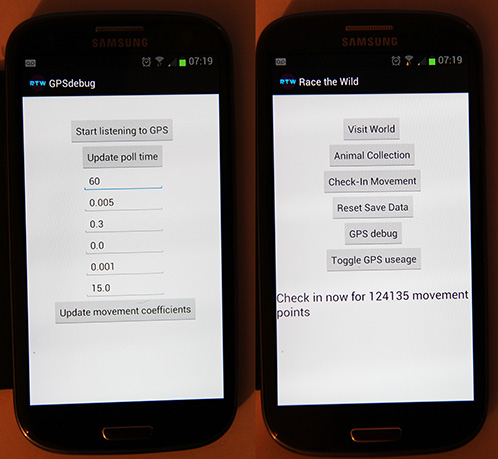
\includegraphics[scale=0.5]{phones.jpg}
\end{center}
\caption{(left to right). 1) GPS debug screen allowing developers to start the AlarmManager, tweak coefficients in the movement point calculation and select how often the GPS should be polled. 2) Main menu screen, showing movement points after quite a significant trip and the ability to turn GPS usage on and off. The ``Toggle GPS usage" button will ultimately be in a more user-friendly position.}
\end{figure}

\subsubsection{Initial testing}
To test that location updates were successful when moving around, the poll time was set to query the GPS every $1$ minute and all coefficients in Equation \ref{eq:mpoints} were set to zero apart from $e$. The actual location was recorded by a separate process and was written along with movement points calculated by the app to a log file. The results are shown in Figure 3.

\begin{figure}
\label{fig:gpstestresults}
\begin{center}
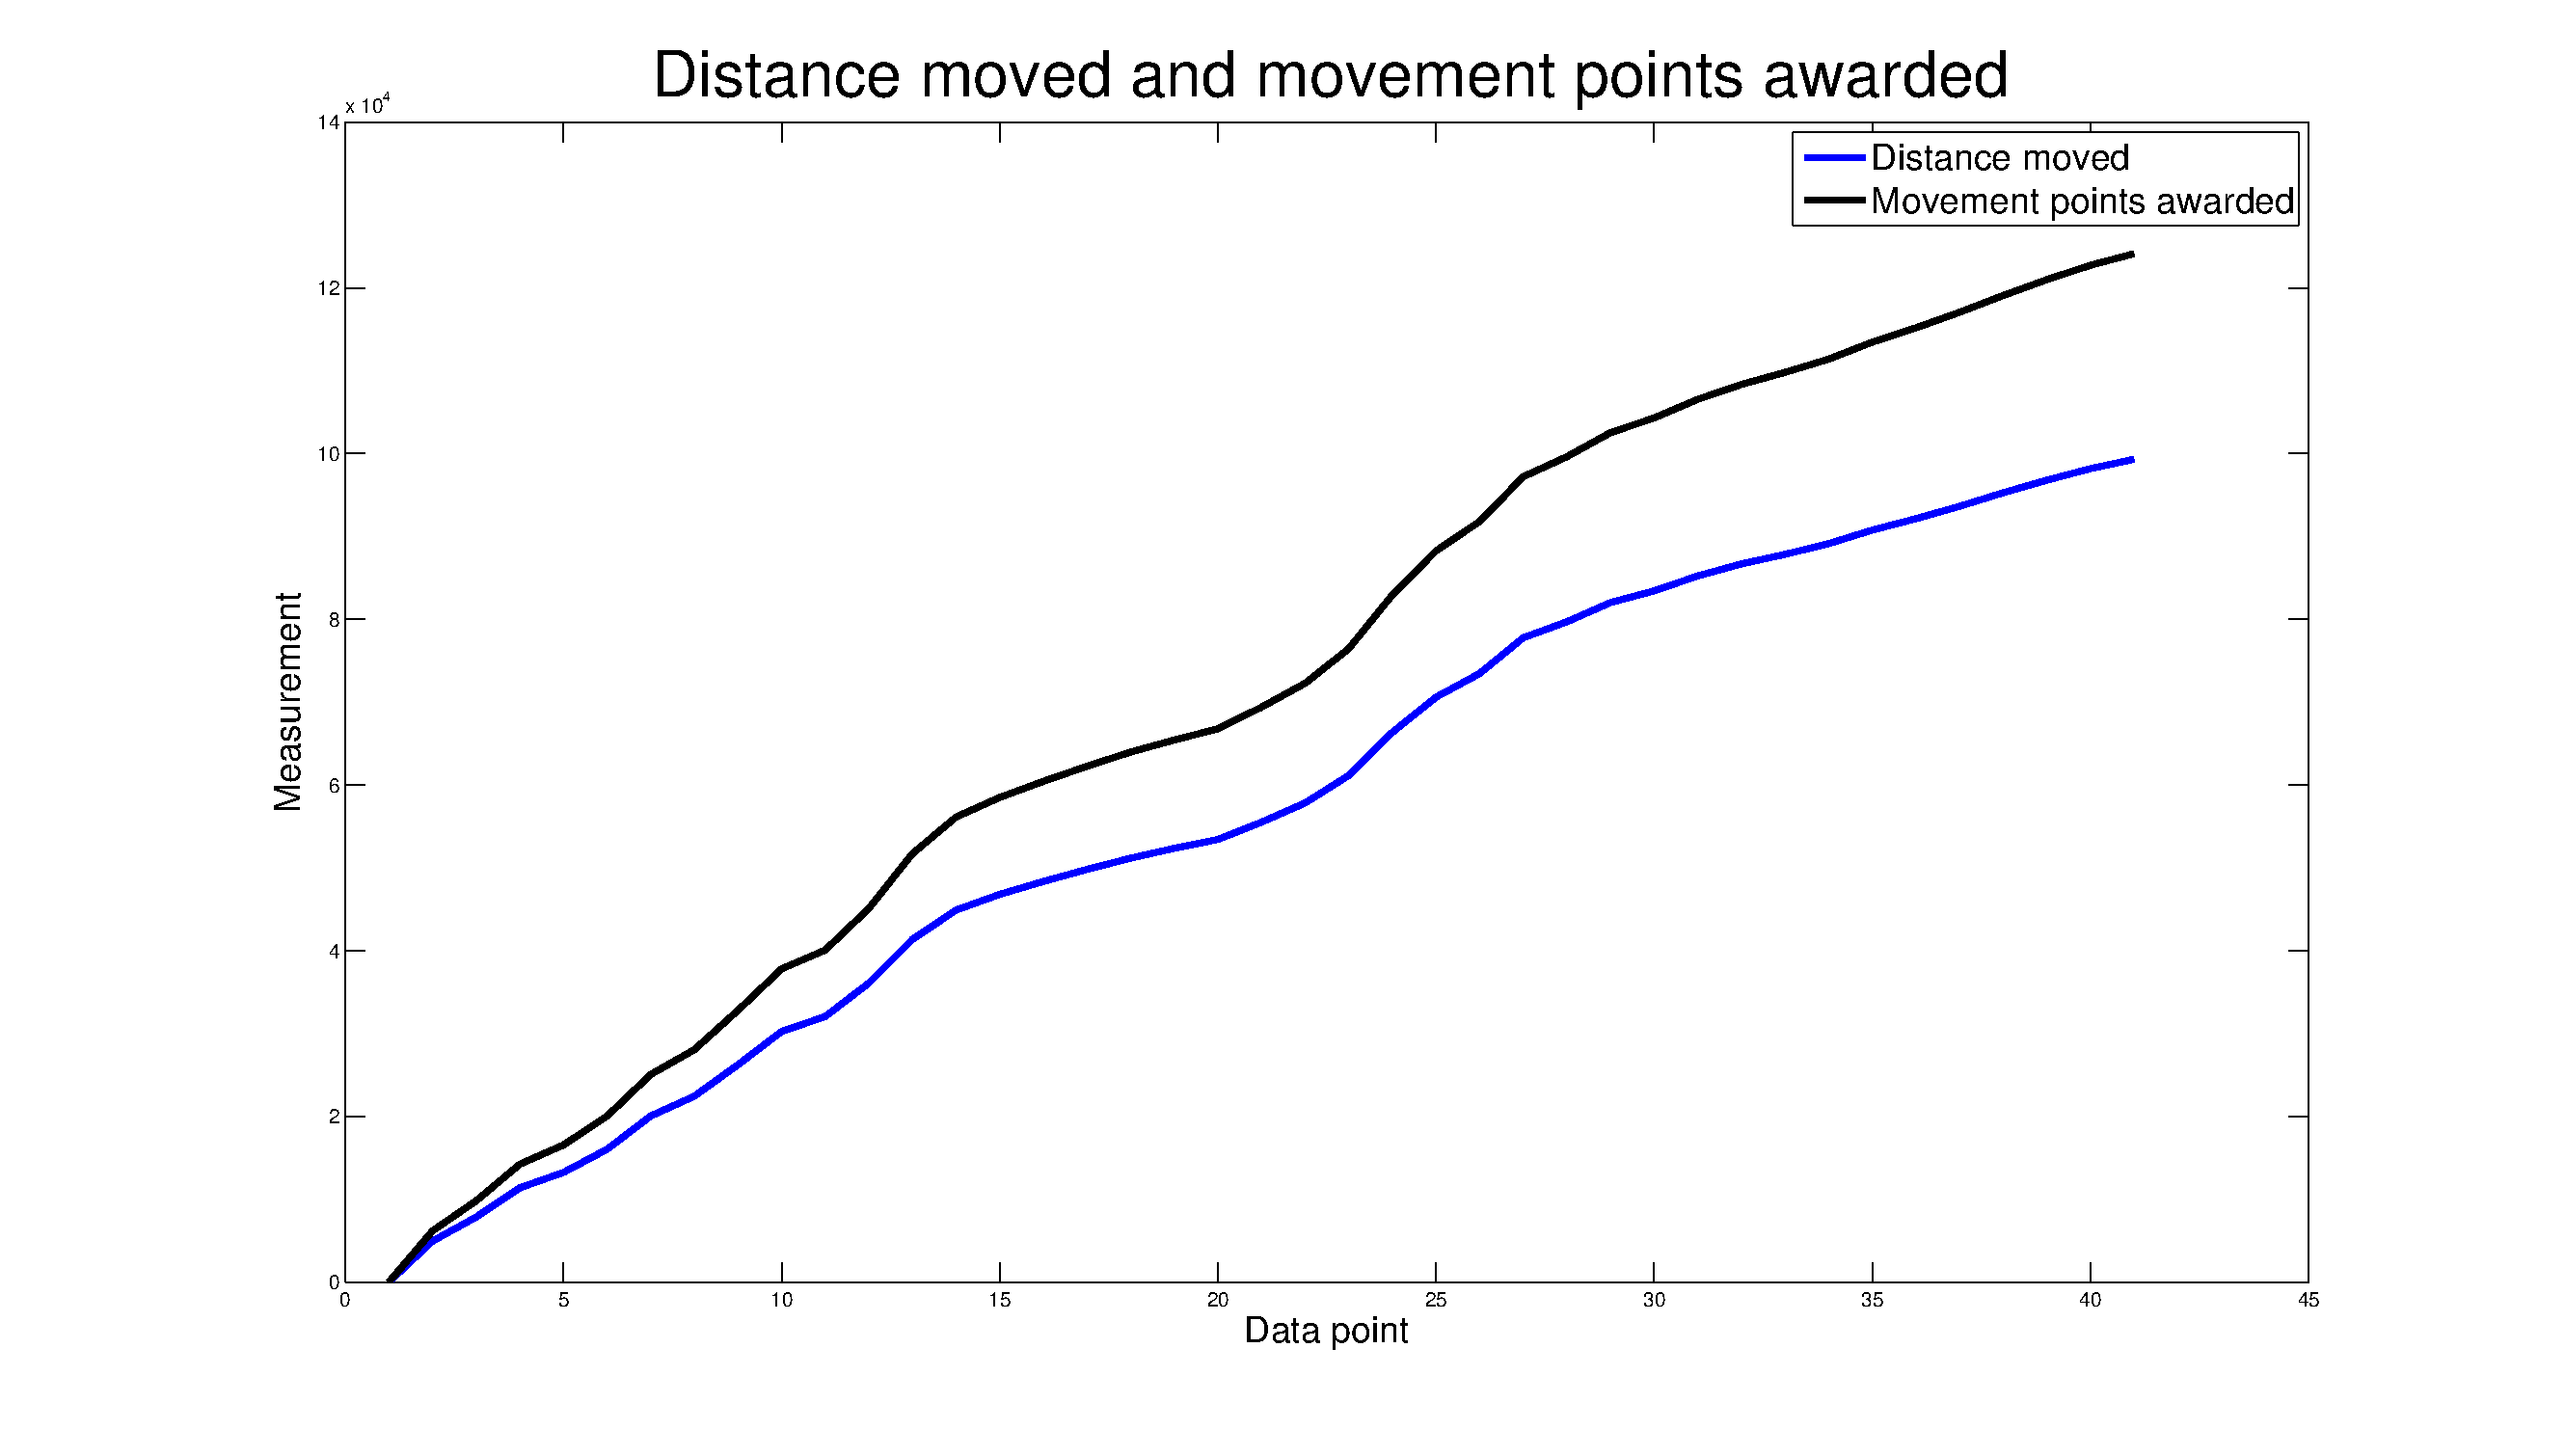
\includegraphics[scale=0.35]{mpoints.eps}
\end{center}
\caption{Testing allocation of movement points as the user moves. Distance is measured in metres. It can be seen that the allocation of movement points using this simple linear relationship ($e$ is the only non-zero coefficient) successfully follows the trend in increasing distance}
\end{figure}

The allocation of movement points follows the increase in distance as the fabricated linear relationship would suggest. The movement points appeared in the main menu screen and the user was allowed to check in to release an animal into the world. The handset usage in this test accurately reflects normal usage - a mixture of being inside and outside buildings, around tall buildings and concurrently using the telephone for voice calls and email.

Over the $2$ hour $40$ minute period that tests were run, the battery capacity on the Samsung Galaxy S$3$ handset upon which the app was running decreased from $90$\% to $75$\%. If, to a first order approximation, all this capacity drainage was as a result of GPS usage (which is clearly flawed since the handset was also used for other tasks concurrently), when the GPS poll period is reduced to $10$ minutes as normal usage would dictate, these initial findings would suggest that the app can be used continually for several days before the battery fully drains.

While GPS updates are incredibly precise and work very well outdoors, getting a fix indoors takes longer and uses more battery. These indoor fixes can also be imprecise, sometimes varying by more than $100$m without any movement having occurred. When indoors, the app incorrectly identified $15$\% of updates as movement when the device had in fact remained stationary. Since the users cannot be expected to turn the location tracking subsystem on and off as they go in and out of buildings, the application should function correctly all the time. A possible solution to the problem is therefore presented in the next section.

\subsubsection{Further work}
Since a user's method of motion tends to stay constant for more than around $20$ minutes (they may be sitting at their desk, riding a bicycle or going for a walk), a sensible way of evading the problem outlined in the previous section regarding occasional spurious GPS readings whilst indoors would be to convolve the vector of distances moved with a vector such as
\[
\left[{ \frac{7}{11},\, \frac{3}{11},\, \frac{1}{11}}\right]
\]
which will mean that when the latest distance reading is recorded, the previous two distance readings are also taken into account. If the user is travelling at a roughly constant speed, then these distances will also be equal, so this convolution would be a reasonable way of smoothing the occasional spurious reading.

Further optimisations can also be made when interacting with the Android API to ensure greater accuracy and greater power efficiency. More testing is also required to ensure that the movement points are correctly calculated when moving at different speeds.

Collaboration is also required with other developers to ensure that the number of movement points allocated for a given movement is of the correct order of magnitude, i.e. it is not too easy or too difficult to release animals and move between nodes in the virtual world.

\subsection{Andrew Sheriff}



\end{document}
